\section{Novos paradigmas}

A integração de inteligência artificial (IA) nas missões espaciais tem aumentado cada vez mais, e com isso, novas oportunidades são compreendidas mas também desafios legais e éticos inéditos surgem. 

\subsection{Inteligência artificial no espaço}

Conforme \cite{martin2021} trata no seu estudo, a IA está transformando as operações espaciais e os desafios regulatórios associados, pois a IA tem aplicações importantes em áreas como processamento de grandes volumes de dados de satélites, navegação autônoma, gerenciamento de detritos espaciais e operações em missões de exploração profunda.
No entanto, a sua adoção também levanta questões críticas relacionadas à responsabilidade, supervisão humana e privacidade \cite{martin2021}.

Uma das principais preocupações é a ausência de um marco regulatório específico para a IA em atividades espaciais.
Embora existam tratados espaciais, como o \cite{unodaOuterSpaceTreaty}, o Tratado do Espaço de 1967 e a Convenção de Responsabilidade de 1972 \cite{camaraDecreto77}, essas diretrizes abordam aspectos gerais e não discorrem sobre os desafios únicos apresentados pela autonomia crescente dos sistemas baseados em IA.

Outro ponto central é o nível necessário de supervisão humana em sistemas equipados com IA.
É discutido por \cite{martin2021} os diferentes modelos de controle, como o controle direto (\emph{human-in-the-loop}), a supervisão indireta (\emph{human-on-the-loop}) e a autonomia completa (\emph{human-out-of-the-loop}), destacando as implicações éticas e legais de cada abordagem.
A supervisão humana, mesmo que reduzida, é vista como essencial para garantir a conformidade com normas internacionais e minimizar os riscos associados à autonomia \cite{martin2021}.

\subsection{Astrobees}

sO \emph{Astrobees} é um sistema robótico desenvolvido pela NASA para operar na ISS, conforme \cite{nasaAstrobee} explica, este dispositivo auxilia os astronautas em tarefas rotineiras e também para explorar novas tecnologias de robótica em microgravidade.
Ao todo são três robôs autônomos denominados como \emph{Honey}, \emph{Bumble} e \emph{Queen}.
O \emph{Astrobee} é um cubo de 31,75 cm de cada lado, e pode funcionar de forma autônoma ou ser controlado remotamente, variando conforme as necessidades da missão.
Eles são capazes de realizar inspeções, monitorar equipamentos, documentar experimentos e transportar pequenos objetos dentro da ISS. Essas ações permitem que os astronautas concentrem seu tempo em atividades mais críticas como as pesquisas a serem desenvolvidas e na manutenção da ISS.

Os \emph{Astrobees} são equipados com sensores e câmeras, além disso, tecnologias avançadas de navegação com visão computacional são usadas para se mover com precisão no ambiente de microgravidade da estação espacial.
O sistema é alimentado por propulsores de ventilador que permitem sua movimentação em todas as direções e ele é capaz de retornar de forma autônoma à sua estação de recarga, o que permite operação contínua e sem intervenção humana direta. Essa capacidade autônoma é suportada por algoritmos de aprendizado de máquina que aprimoram sua eficiência ao longo do tempo \cite{nasaAstrobee}.

\begin{figure}
    \centering
    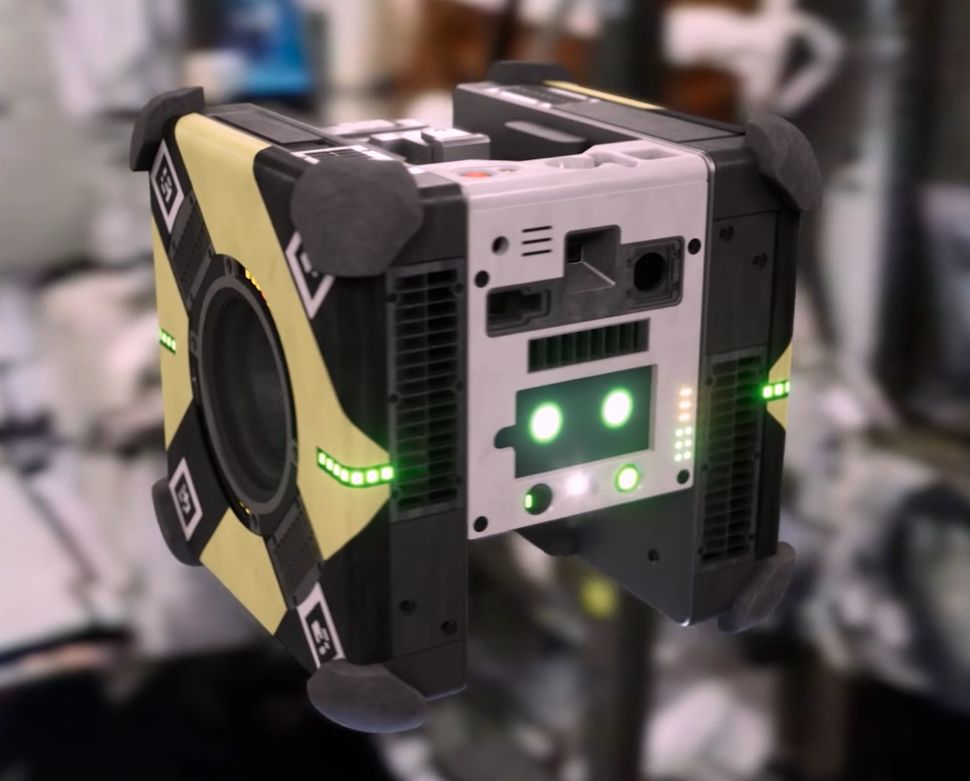
\includegraphics[width=0.75\linewidth]{1 Introducao/Imagens/Astrobee NASA.png}
    \caption{Astrobee, robô auxiliar dos pesquisadores na ISS. Fonte: Space.com.}
    \label{fig:AstrobeeFoto}
\end{figure}

Adicionalmente, os \emph{Astrobees} servem como uma plataforma de teste para novas tecnologias espaciais. Os pesquisadores podem carregar e testar software personalizado nos robôs para simular cenários de futuras missões espaciais para desenvolver soluções para operações em estações espaciais futuras como o \emph{Lunar Gateway}, que será utilizada em missões no espaço profundo \cite{nasaAstrobee}.

\subsection{Acoplamento autônomo da Dragon 2}

A espaçonave Dragon 2, cujo desenvolvimento foi iniciado no primeiro semestre de 2013 pela SpaceX \cite{spaceDragonAlien}, é projetada para transportar tanto cargas quanto tripulações humanas ao espaço.
Essa versão se baseia no modelo original \emph{Dragon 1} e apresenta melhorias em termos de autonomia, segurança e capacidade operacional.
A \emph{Dragon 2} pode transportar até sete tripulantes ou uma combinação de cargas e tripulantes, podendo ser utilizada em diferentes tipos de missões espaciais, como o transporte para a ISS ou a entrega de novos astronautas na ISS para que outros retornem para a Terra.

Entre as principais melhorias em relação à \emph{Dragon 1}, está o sistema de lançamento e retorno. A \emph{Dragon 2} é equipada com motores \emph{SuperDraco}, que oferecem capacidade de abortagem de emergência durante o lançamento.
Esse sistema permite que a espaçonave escape em caso de falhas no foguete, protegendo a tripulação. Além disso, a \emph{Dragon 2} utiliza paraquedas redesenhados para garantir um pouso mais controlado, uma atualização em relação ao modelo anterior, que dependia de procedimentos diferentes para retornar à Terra.
Outra inovação é o sistema de navegação autônoma \cite{nasaStarshipDocking}, que realiza o acoplamento direto à ISS sem a necessidade do braço robótico \emph{Canadarm2}, que em sua versão anterior (\emph{Dragon 1}) exigia para realizar o acoplamento na ISS.
Essa funcionalidade reduz melhora a eficiência das missões pois eleva a segurança, reduz a dependência humana e pode ocorrer mesmo que haja restrições como ausência de iluminação ou tripulação em horário de descanso.
Por fim, a \emph{Dragon 2} apresenta um design interno atualizado, com controles interativos por \emph{touchscreen} e maior conforto para longas viagens.

\subsection{Sustentabilidade}

À medida que o número de objetos em órbita aumenta, a estabilidade do ambiente operacional se torna uma preocupação cada vez maior.
Nos últimos anos, uma grande quantidade de detritos espaciais se acumulou com os satélites e espaçonaves inseridas no espaço, trazendo risco para futuras missões e para a integridade das operações atuais.
O lixo espacial varia de grandes pedaços de foguetes desativados a detritos de colisões e explosões em órbita.
É estimado que existam mais de 670.000 objetos maiores que 1 cm na órbita da Terra \cite{esaSpaceDebris}, e outros milhões de objetos menores representando sérios riscos.
O problema é agravado pelo uso de satélites de órbita baixa, como os projetos \emph{Starlink} e \emph{OneWeb}, que prometem melhorar a conectividade e comunicação global pela internet sem restrições de localização.
Os impactos que acontecem em alta velocidade, conforme explica \cite{esaAboutSpaceDebris}, podem criar milhares de fissuras, levando a um problema maior e a uma condição conhecida como síndrome de Kessler, onde colisões acontecem em cascata e se propagam sequencialmente, causando a inutilização de certas órbitas por muitos anos ou até séculos \cite{kessler1978}.

Além dos riscos de colisões, os locais de resíduos também trazem impactos financeiros e operacionais. As empresas espaciais privadas e as agências espaciais enxergam a necessidade de investir em manutenção preventiva para proteger suas espaçonaves.
Ao desviarem dos detritos, os custos operacionais são aumentados pois elevam o consumo de propelente e encurtam a vida útil do satélite.
Por outro lado, a falta deste gerenciamento de detritos pode danificar ativos e levar a interrupções, causando fissuras econômicas na indústria orbital.

A gestão de resíduos demanda cooperação internacional.
Medidas como a coleta de objetos por robôs de captura e a implementação de padrões mais rigorosos para remoção de satélites são passos importantes para redução do problema.
Organizações como a ESA e a NASA também estão promovendo projetos sustentáveis \cite{esaDebrisMitigation2023}; elas estão incentivando o uso de materiais que queimam completamente na reentrada.

\subsection{MEV}

O \emph{Mission Extension Vehicle-1} (MEV-1), desenvolvido pela \emph{Northrop Grumman}, é uma espaçonave projetada para estender a vida útil de satélites em órbita geossíncrona.
Lançado em 9 de outubro de 2019, o \emph{MEV-1} realizou sua primeira missão em fevereiro de 2020, ao se acoplar a um satélite alvo (\emph{Intelsat 901}), conforme explicado por \cite{nytMEV1}. O objetivo era estender a vida útil da missão do  alvo.
Em abril de 2025 a missão foi encerrada, quando o \emph{MEV-1} moveu o alvo para uma órbita cemitério \cite{intelsat901}.
O \emph{MEV-1} utilizou um mecanismo de captura que se conectou ao motor principal do satélite alvo para assumir o controle de suas operações de atitude e órbita.
Essa tecnologia permite que satélites que seriam desativados continuem em operação, reduzindo a necessidade de lançar novos satélites e contribuindo para a sustentabilidade das operações espaciais.
Além de sua capacidade de extensão de vida útil, o \emph{MEV-1} demonstra avanços em operações de proximidade e acoplamento em órbita. Isso contribui para os serviços de manutenção espacial \cite{mev1}.

\subsection{Missões de exploração}

O programa \emph{Artemis}, liderado pela NASA, busca estabelecer uma presença sustentável ao redor da Lua e em sua superfície \cite{nasaArtemis}.
Isso requer o desenvolvimento de tecnologias avançadas para operações de \emph{RVD/B} em ambientes altamente conectados.
Ao contrário das operações em órbita baixa da Terra, as missões lunares apresentam desafios únicos pois a distância entre a Lua e a Terra pode causar atrasos nas comunicações de alguns segundos \cite{keeports2006}.
Isso limita o controle humano imediato e exige sistemas autônomos robustos e confiáveis para execução do acoplamento entre as espaçonaves e os módulos espaciais.

Para transpassar essas limitações, os sistemas de \emph{RVD/B} na superfície lunar são usados com autonomia robótica aprimorada para que eles possam realizar os procedimentos de forma independente.
Sensores como o LiDAR \cite{farkasvolgyi2023} e câmeras estereoscópicas, combinados com algoritmos de aprendizado de máquina e processamento de dados em tempo real permitem que as espaçonaves detectem objetos \cite{ibmComputerVision}.
Com isso, podem calcular trajetórias de aproximação sem falha e sem a necessidade imediata da gerência de solo.

A tecnologia desenvolvida para o programa \emph{Artemis} tem aplicações diretas em futuras missões de exploração a Marte e outras partes do sistema solar que terão uma missão de vida útil muito mais longa.
A integração de sistemas autônomos de \emph{RVD/B} representa um avanço nas capacidades humanas de operar em ambientes espaciais desafiadores, obtendo um equilíbrio entre sustentabilidade e na redução da dependência de intervenções diretas pelos humanos.